\chapter{Theory}\label{cha:theory}

\begin{comment}
The background theory depth and breadth depend on the depth needed to understand your project
in the different disciplines that your project crosses.
It is not a place to just write about everything you know that is vaguely connected to your project.
The theory is here to help the readers that do not know the theoretical basis of your work so that they
can gain sufficient understanding to understand your contributions --- and also for yourself to show that
you have understood the underlying theory and are aware of the methods used in the field.
In particular, the theory section provides
an opportunity to introduce terminology that can later be used without disturbing the text with a definition.
In some cases it will be more appropriate to have a separate section for different theories (or even separate chapters).
However, be careful so that you do not end up with too short sections.
Subsections may also be used to separate different background theories.

Be aware that ``background'' is a general term that refers to everything done by somebody else,
in contrast to the ``foreground'', which is your own work.
Hence there can (and will) be several background chapters, with the background theory being one of them
--- or several of them, since it thus is quite possible to split the background theory over more than one chapter,
e.g., by having a chapter introducing the theory directly needed for the research field in question and another
chapter discussing the machine learning theory, algorithms, tools, and evaluation methods commonly used in the field.
The related work chapter is thus also part of the background, while a chapter about data might be background
(if you only use somebody else datasets), but can also be part of the foreground (if you collect and/or annotate data
yourself, or if you process or clean the data in ways that can make it part of your own contribution).

It is ok to reuse material from other texts that you have written (e.g., the specialisation project), but if you do so, that must be clearly stated in the text, together with a description of how much of the text is new, old or rewritten/edited.
Such a statement about recycling of material in the Background Theory chapter can thus come here in the chapter introduction.

\section{Writing References in the Text}
\label{sec:writing_references}

When introducing techniques or results, always reference the source.
Be careful to reference the original contributor of a technique and not just someone who happens to use the technique.%
\footnote{But always make sure that you have read the work you are citing --- if not, cite someone who has!}
For results relevant to your work,
you would want to look particularly at newer results so that you have referenced the most up-to-date work in your area.
A common rule of thumb is to at least reference the first paper introducing the issue and the paper containing the latest / state-of-the-art
results. Additional papers making substantial contributions should also be referenced, as well as of course the ones you find most interesting.
Remember to use the right verb form depending on the number of authors.

If you do not have the source handy when writing, mark in the text that a reference is needed and add it later. \todo{add reference}
Web pages are not reliable sources --- they might be there one day and removed the next; and thus should be avoided, if possible.
A verbal discussion is not a source and should normally not be referenced
(though you can reference ``personal communication'', if there are no other options).
The bulk of citations in the report will appear in Chapter~\ref{cha:related_work}.
However, you will often need to introduce some terminology and key citations already in this chapter.

You can cite a paper in the following manner (and several other versions,
see the \verb!natbib! package documentation):

\section{The Reference List}
\label{sec:reference_list}

In general, make sure that the references that appear in your reference list can be easily located and identified by the reader.
So include not only authors and title, but year and place of publication, the full names of conferences and workshops,
page numbers in proceedings and collections, etc.
Hyperlinks or \acrfull{acr:doi} numbers are also nice to include.
Just as in the text itself, it is important to be consistent in the reference list, so include the same type of information for all references and write it in the same way.

% Check out the reference list at the end of this document for examples of how to write references in \BibTeX.
% Note a particular quirk: Many \BibTeX\ styles convert uppercase letters to lowercase, unless specifically told not to.
% You might thus need to ``protect'' characters that should not be converted, e.g., by writing \texttt{\{T\}witter} as in the \citet{FountaEA:18} reference.

% Also, keep in mind that `et' is a word in its own right (`and'), so there is no period after it (even though there is a period after `al.', which is short for `alia', meaning `others').
% Of course, when including such a reference in the text, the authors should be referred to in plural form. 
% So \citet{BenyonEA:13} state that life is good (not ``states'').

% Many sites, such as journals and \url{dblp.org} provide the matching \BibTeX\ entry for a reference. 
% However, you might still need to edit the entry in order to be consistent with the rest of your references.
% If you find references from sites such as \url{scholar.google.com} or \url{arXiv.org}, keep in mind that they often not are complete,
% so that you might need to add information to the entry (and probably edit it as well).

Some other good sites to find state-of-the-art work:
\begin{itemize}
    \item \url{paperswithcode.com}
    \item \url{nlpprogress.com}

\end{itemize}

\textit{Lorem ipsum dolor sit amet, consectetur adipiscing elit, sed do eiusmod tempor incididunt ut labore et dolore magna aliqua. Ut enim ad minim veniam, quis nostrud exercitation ullamco laboris nisi ut aliquip ex ea commodo consequat. Duis aute irure dolor in reprehenderit in voluptate velit esse cillum dolore eu fugiat nulla pariatur. Excepteur sint occaecat cupidatat non proident, sunt in culpa qui officia deserunt mollit anim id est laborum.}


\section{Introducing Figures}

\LaTeX is a bit tricky when it comes to the placement of ``flooting bodies'' such as figures and tables. It is often a good idea to let their code appear right before the header of the (sub)section in which they appear.
Note that you should anyhow always use an option for the placement (e.g., \verb|[t!]| to place it at the top of a page).

Do not just put the figure in and leave it to the reader to try to understand what the figure is.
The figure should be included to convey a message and you need to help the reader to understand the message
intended by explaining the figure in the text.
Hence \textbf{all} figures and tables should always be referenced in the text, using the \verb!\ref! command.
It is good practice to always combine it with a non-breakable space (\verb!~!) so that there will be no newline between the term referring to it and the reference, that is, using \verb!Figure~\ref{fig:BoxesAndArrowsAreNice}!.

Also, note that you can have a longer version of the figure (and table) caption attached to the actual figure,
while using the optional first argument to \verb!\caption! to include a shorter version in the list of figures (lof) or list of tables:
\begin{quote}
    \begin{verbatim}
\caption[Shorter lof text]{Longer text appearing under the figure}
\end{verbatim}
\end{quote}

\begin{figure}[t!]
    \centering
    \missingfigure{Here we will add an amazing figure explaining it all}
    \caption{A missing figure}
    \label{fig:AmazingFigure}
\end{figure}

In general it is good to add notes about things that you plan on writing later.
The \verb!todonotes! package is great for that kind of book-keeping, letting you write both shorter comments in the margin\todo{l8r dude} and longer comments inside the text, using the option \verb![inline]!.
\todo[inline]{There are always some more stuff that you will need to add at some later point.
    Be sure to at least make a note about it somewhere.}

\textit{Sed ut perspiciatis unde omnis iste natus error sit voluptatem accusantium doloremque laudantium, totam rem aperiam, eaque ipsa quae ab illo inventore veritatis et quasi architecto beatae vitae dicta sunt explicabo. Nemo enim ipsam voluptatem quia voluptas sit aspernatur aut odit aut fugit, sed quia consequuntur magni dolores eos qui ratione voluptatem sequi nesciunt. Neque porro quisquam est, qui dolorem ipsum quia dolor sit amet, consectetur, adipisci velit, sed quia non numquam eius modi tempora incidunt ut.}

\section{Introducing Tables in the Report}

\newcommand\emc{-~~~~}
\begin{table}[t!]
    \centering
    \caption[Example table]{Example table (F$_1$-scores); this table uses the optional shorter caption that will appear in the list of tables, so this long explanatory text will not appear in the list of tables and is only here in order to explain that to the reader.}
    \begin{tabular}{c|c|rrrrrr}
        \tabletop
        Langs                  & Source                                           & \multicolumn{1}{c}{Lang1} & \multicolumn{1}{c}{Lang2} & \multicolumn{1}{c}{Univ} & \multicolumn{1}{c}{NE} & \multicolumn{1}{c}{Mixed} & \multicolumn{1}{c}{Undef}
        \\ \tablemid
        \multirow{5}{*}{EN-HI} & FB+TW                                            & 54.22                     & 22.00                     & 19.70                    & 4.00                   & 0.05                      & 0.03                      \\
                               & FB                                               & 75.61                     & 4.17                      & 18.00                    & 2.19                   & 0.02                      & 0.01                      \\
                               & TW                                               & 22.24                     & 48.48                     & 22.42                    & 6.71                   & 0.08                      & 0.07                      \\
                               & Vyas                                             & 54.67                     & 45.27                     & 0.06                     & \emc                   & \emc                      & \emc                      \\
                               & FIRE                                             & 45.57                     & 39.87                     & 14.52                    & \emc                   & 0.04                      & \emc                      \\ \tablemid
        \multirow{2}{*}{EN-BN} & TW                                               & 55.00                     & 23.60                     & 19.04                    & 2.36                   & \emc                      & \emc                      \\
                               & FIRE                                             & 32.47                     & 67.53                     & \emc                     & \emc                   & \emc                      & \emc                      \\ \tablemid
        EN-GU                  & FIRE                                             & 5.01                      & \textbf{94.99}            & \emc                     & \emc                   & \emc                      & \emc                      \\
        \tablemid
        DU-TR                  & Nguyen                                           & 41.50                     & 36.98                     & 21.52                    & \emc                   & \emc                      & \emc                      \\ \tablemid

        EN-ES                  & \multirow{4}{*}{\rotatebox[origin=c]{90}{EMNLP}}
                               & 54.79                                            & 23.50                     & 19.35                     & 2.08                     & 0.04                   & 0.24                                                  \\
        EN-ZH                  &                                                  & 69.50                     & 13.95                     & 5.88                     & 10.60                  & 0.07                      & \emc                      \\
        EN-NE                  &                                                  & 31.14                     & 41.56                     & 24.41                    & 2.73                   & 0.08                      & 0.08                      \\
        AR-AR                  &                                                  & 66.32                     & 13.65                     & 7.29                     & 11.83                  & 0.01                      & 0.90                      \\ \tablebot
    \end{tabular}
    \label{tab:ExampleTable}
\end{table}

As you can see from Table~\ref{tab:ExampleTable}, tables are nice.
However, again, you need to discuss the contents of the table in the text.
You do not need to describe every entry, but draw the reader's attention to what is important in the table,
e.g., that 94.99 is an amazing F$_1$-score (and that probably something fishy happened there).
Use boldface, boxes, colours, arrows, etc. to mark the important parts of the table.

As can be seen in the example, elements in a table can sometimes benefit from being rotated (such as EMNLP in the `Source' column) or cover more than one row (EMNLP, as well as EN-HI and EN-BN in the `Langs' column) --- or more than one column, for that matter.
\end{comment}

\Autochapterref{cha:theory} of this specialization project will talk about the leading technologies in the field of \gls{acr:llm}, which in itself is a subfield of \gls{acr:nlp}. \autoref{sec:llms} will go over the leading \gls{acr:llm} models, their strengths and weaknesses, and briefly mention differences in model architecture. \Autosectionref{sec:llm-providers} will name the most prominent providers of \gls{acr:llm} services.

\autoref{fig:actor-map} shows an actor map which includes stakeholders, providers, and other groups and organizations that could have some relevance to an autonomous LLM-based GIS-agent. Following subsections will go over the different groups and explain why they are included in the actor map.

\begin{figure}
    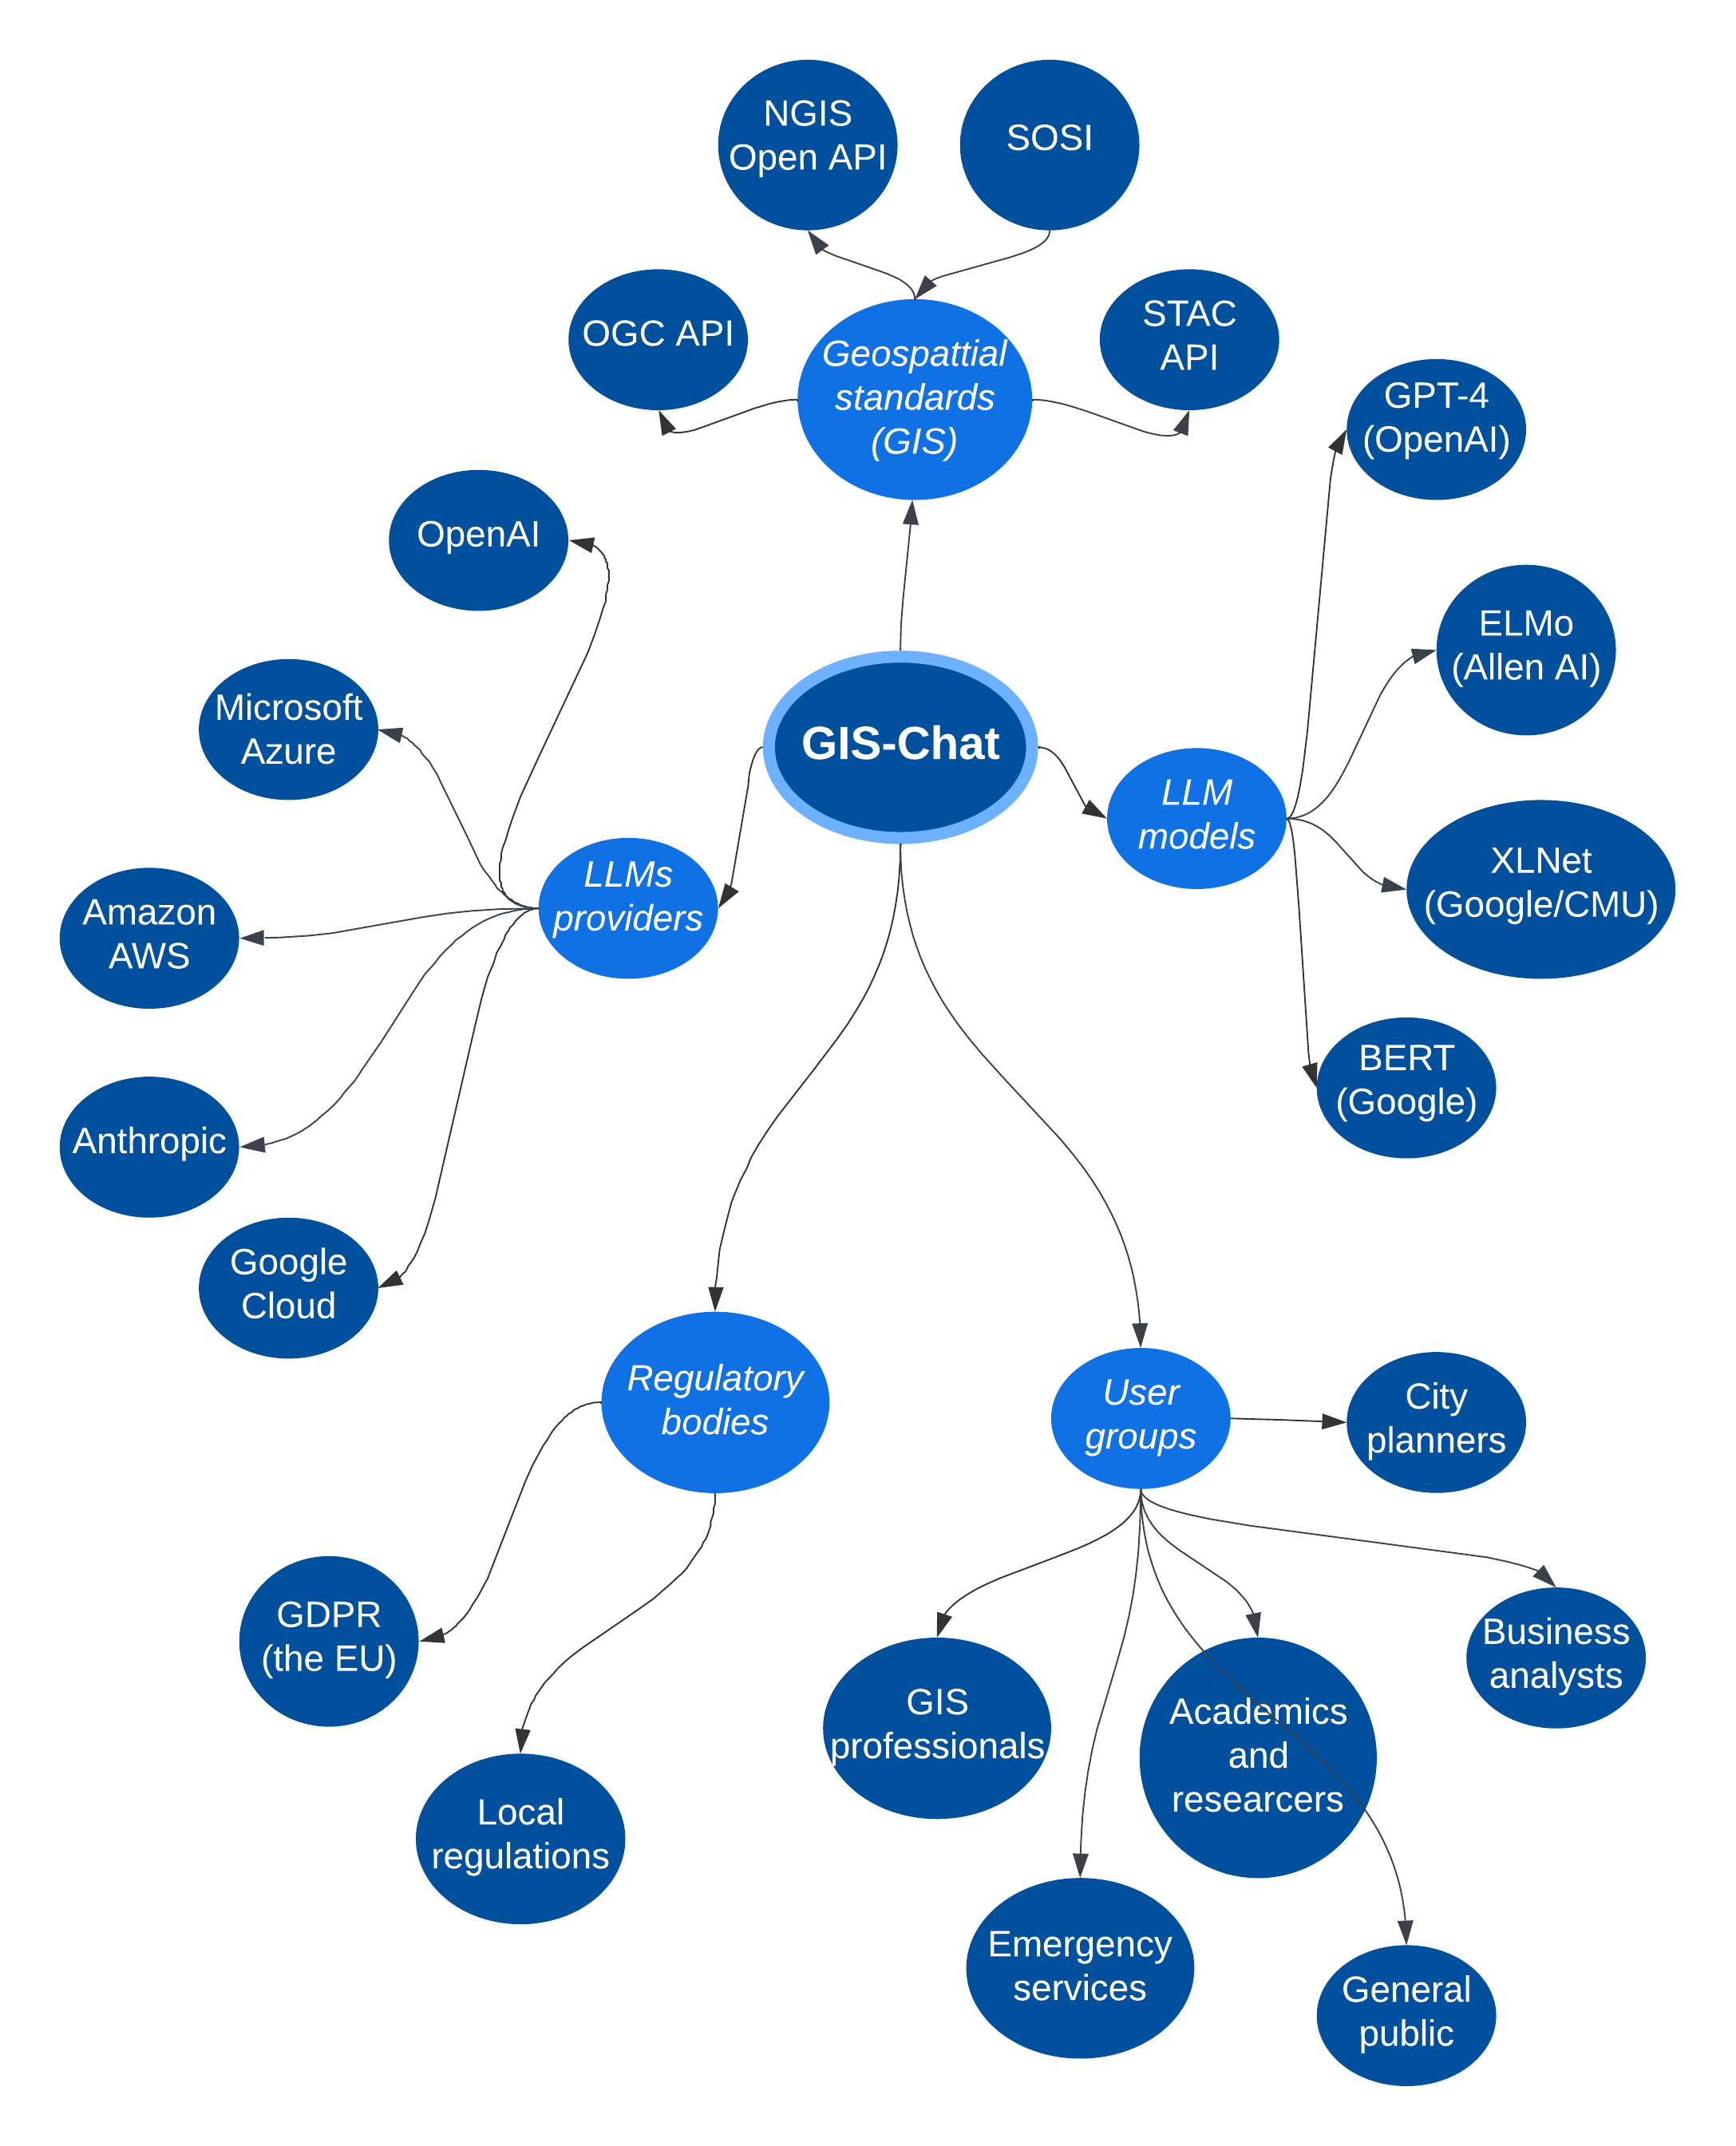
\includegraphics[width=\textwidth]{actor_map}
    \caption{Actor map for stakeholders, providers, and other groups and organizations that could have some relevance to an autonomous LLM-based GIS-agent.}
    \label{fig:actor-map}
\end{figure}

\section[Large Language Models]{\acrshortpl{acr:llm}}\label{sec:llms}

\subsection[The GPT Family]{The \acrshort{acr:gpt} Family}

\glspl{acr:gpt} are a type of \gls{acr:llm} first introduced by \hyperref[subsec:openai]{OpenAI} in 2018 \citep{radfordImprovingLanguageUnderstanding2018}.

\subsection[The BERT Family]{The \acrshort{acr:bert} Family}

\gls{acr:bert} is a family of language models developed at Google \citep{devlinBERTPretrainingDeep2019}, first presented in 2018.

\subsection{Google Products}

\subsubsection{PaLM 2}

\subsubsection{Codey}

\section[LLM providers]{\acrfull{acr:llm} Providers}\label{sec:llm-providers}

\subsection{OpenAI}\label{subsec:openai}

Being the most widely famous actor within the field of \glspl{acr:llm}, OpenAI has gained great influence through their vast portfolio.

\subsection{Microsoft Azure}\label{subsec:microsoft-azure}

\subsection{Google Cloud}\label{subsec:google-cloud}

\subsection[Amazon Web Services (AWS)]{\acrlong{acr:aws}}\label{subsec:aws}

\subsection{Anthropic}\label{subsec:anthropic}

\section{Geospatial Standards}\label{sec:geospatial-standards}

\subsection{International Standardization Work}\label{subsec:standardization-international}

\subsubsection[OGC Standards]{\acrshort{acr:ogc} Api Standard}\label{subsubsec:ogc}

The \gls{acr:ogc} \acrshort{acr:api} Standards serve as the glue in the field of \gls{acr:gis}, paving the way for interoperability and data exchange between diverse systems. Leveraging common web protocols like \acrshort{acr:html} and supporting multiple data formats including \acrshort{acr:json}, \acrshort{acr:gml}, and \acrshort{acr:html}. The \gls{acr:ogc} \acrshort{acr:api} standard provides a modular architecture consisting of a core specification and various extensions. This modularity allows for flexibility, enabling users to customize their services according to specific needs. According to their webpages, they provide 80 different standards, each for a specific geospatial purpose. Notable examples are 3D Tiles, CityGML, GeoTiff, and \acrshort{acr:ogc} \acrshort{acr:api} - Features \citep{ogcOGCStandards2023}.

\acrshort{acr:ogc} \acrshort{acr:api} Standards function as modern replacements to older standards like \acrshort{acr:wms} and \acrshort{acr:wfs}, and presents an evolved and more adaptable framework for spatial data operations, setting the stage for future innovations in the \acrshort{acr:gis} domain.

\subsubsection[STAC Api Standard]{\acrshort{acr:stac} Api Standard}\label{subsubsec:stac}

The \gls{acr:stac} \acrshort{acr:api} is a standardized way to expose collections of spatial temporal data for online search and discovery. Built upon a \acrshort{acr:json} core, it aims to be a uniform and flexible environment from which developers can customize the API infrastructure to their domain. \gls{acr:stac} \acrshort{acr:api} provides a powerful query language that allows users to search by various parameters like time, location, and keywords, making widely applicable. The \acrshort{acr:stac} community has also defined specification in order remove the complexity associated with having to create unique pipelines when consuming different spatial-temporary collection. The significance of the \gls{acr:stac} \acrshort{acr:api} lies in its ability to democratize access to large volumes of geospatial data. By offering a common standard for data cataloguing and discovery, it reduces the barriers that often exist due to incompatible data formats. Developers or \acrshort{acr:gis} professionals can take advantage of this through built-in tooling in QGIS, a desktop \gls{acr:gis} for viewing, editing, and analysing spatial data, or through third-party packages in the Python and R programming languages. The API is also accessible through the command line interface when using \acrshort{acr:gdal} \citep{STACTutorials}.

As \acrshort{acr:ogc} board member Chris Holmes puts it: "The \acrshort{acr:stac} \acrshort{acr:api} implements and extends the \gls{acr:ogc} \acrshort{acr:api} — Features standard, and our shared goal is for \gls{acr:stac} \acrshort{acr:api} to become a full \gls{acr:ogc} standard." \citep{holmesSpatioTemporalAssetCatalogs2021}.

\subsection{Norwegian Standardization Work}\label{subsec:standardization-norway}

Geospatial standardization work has been on the agenda of Norwegian governing powers for decades and have materialized in frameworks/collaborations like \nameref{subsubsec:geovekst} and \nameref{subsubsec:norge-digitalt}, as wells as the \nameref{subsubsec:sosi} file format. \Autosubsectionref{subsec:standardization-norway} will delve into the work that has been done and what is expected for the future. The reasoning for the conclusion of this section is that the constraints of this specialization project is set by the Norwegian borders, and thus it is important to be aware of the standards that apply.

\subsubsection[SOSI]{\acrshort{acr:sosi}}\label{subsubsec:sosi}

\gls{acr:sosi} is a Norwegian file format for storing and exchanging geospatial data. It was first introduced in 1987 and has since approached international standards, the most important arenas currently being \acrshort{acr:iso}/\acrshort{acr:tc} 211 and \gls{acr:ogc} \citep{mardalNasjonalStrategiVidereutvikling2015}. \gls{acr:sosi} is the adopted Norwegian standard for creating and delivering digital geographic data, administered by the Norwegian Mapping Authority (Statens kartverk) \citep{maehlumSOSI2023}.

In a \gls{acr:sosi} dataset, terrain points, lines, and polygons are represented by their coordinates and classified into various object types according to the \gls{acr:sosi} object catalog standard. However, there are few GIS systems that can read \gls{acr:sosi} data directly, so data in \gls{acr:sosi} format usually needs to be converted to another \gls{acr:gis}-readable data format \citep{maehlumSOSI2023}.

\subsubsection{Geovekst}\label{subsubsec:geovekst}

Geovekst is a collaborative initiative in Norway aimed at collecting, managing, and distributing geospatial information. Established in 1992, it is a partnership between national, regional, and local government bodies, as well as several private companies. Geovekst's primary focus is on creating a comprehensive, standardized geographical database for Norway that is easily accessible and updated regularly. It has played a vital role in various planning and development projects across the country, from urban planning to environmental conservation.

Unlike other geospatial initiatives, Geovekst emphasizes shared responsibilities and costs among its partners. This cooperative model ensures consistent data quality and efficient use of resources. It utilizes a variety of data sources, including aerial photographs, laser scans, and mapping, making it a rich resource for both public and private sectors. Moreover, its open-access policy allows for wider dissemination of geospatial information, thus encouraging innovation and informed decision-making across multiple disciplines.

\subsubsection{Norge digitalt}\label{subsubsec:norge-digitalt}

Established in 2005, Norge Digitalt is a more recent framework compared to Geovekst and is the name of Norway's national spatial data infrastructure. Norge Digitalt primarily involves governmental bodies (national, regional, and municipal), but also educational and research institutions and companies with responsibilities on a nation-wide scale; examples include Telenor and local and regional energy companies \citep[6]{norgedigitaltGenerelleVilkarNorge2023}. Norge Digitalt aims to coordinate and streamline all geospatial activities in Norway, making it easier for users to discover, access, and use spatial data.

One key feature of Norge Digitalt is its focus on international standards and interoperability. While Geovekst is primarily a national initiative, Norge Digitalt aims to integrate Norway's geospatial data with that of other European countries. It supports a wide range of data formats and follows international standards, including those set by the Open Geospatial Consortium (OGC). The framework also provides various tools and services, like metadata catalogues and web services, making it a comprehensive solution for geospatial data management and distribution in Norway.

\section{User Groups}\label{sec:user-groups}

There are several user groups that could take advantage of an \acrshort{acr:ai}-based agent with general geographic and \acrshort{acr:gis} knowledge. Questions can span from simple retrieval questions such as "How many people live in Trondheim" and "How long is the drive from Oslo to Bergen?", to more complicated questions that require problem-solving abilities and reasoning. While it is difficult to obtain dataset over common queries, \cite{kumarWhatArePeople2023a}, creater of the chatbot app Pocket AI\footnote{\url{https://github.com/varunon9/pocket-ai}}, shared a dataset of \textasciitilde 13k user queries from his app along with classifications of these. Salient categories were:

\begin{itemize}
    \item "task oriented" (23.1\%)
    \item "informational" (20.2\%)
    \item "social"  (16.2\%)
    \item "personal advice and self-improvement" (13.1\%)
\end{itemize}

The main takeaway from these numbers is that the main motivation for use is productivity.

This aligns with the results of \cite*{skjuveWhyPeopleUse2023} from their questionnaire-based study performed in late January 2023, about three months after its release \citep{openaiGPT4TechnicalReport2023}. The goal with the study was to find out \textit{why} people use ChatGPT. They found that most participants (55\%) are motivated by productivity, and specifically applying it for routine tasks, information retrieval, text generation and writing support, and software development \citep[17-21]{skjuveWhyPeopleUse2023}. \autoref{tbl:chatgpt-motivation-survey-restuls} shows all categories and their frequencies. There were 197 samples in total, and more than one category could be  assigned to each sample. It is worth noting that the study is likely to have included early adopters, and might therefore make the results less representative for the time at which this report is written (\today), now that use patterns have become more established \citep[37]{skjuveWhyPeopleUse2023}.

\begin{table}[ht]
    \centering
    \caption{Categories and frequency of ChapGPT usage \citep[16-17]{skjuveWhyPeopleUse2023}.}
    \label{tbl:chatgpt-motivation-survey-restuls}
    % \begin{tabular}{|B|c|}
    \begin{tabular}[t]{lr}
        \hline
        \textbf{Category}              & \% \textbf{(n)} \\
        \hline
        Productivity                   & 55\% (109)      \\
        Novelty                        & 51\% (101)      \\
        Fun and amusement              & 20\% (41)       \\
        Creative work                  & 18\% (34)       \\
        Social interaction and support & 9\% (18)        \\
        Other                          & 7\% (15)        \\
        \hline
    \end{tabular}
\end{table}

Given that the main reason people use conversational \acrshort{acr:ai} is for productivity, whether in a professional, academic, or personal context, such technology could be highly beneficial in a geospatial setting. 67 out of the 197 participants in \cite[18]{skjuveWhyPeopleUse2023} highlighted "ChatGPT's ability to understand complex queries" and that it is "efficient in alleviating the need to experiment with different phrasings of the query", as is often needed when 'Googling' for an answer to a specific question. This ease of information retrieval, along with it's problem-solving abilities \citep[20]{skjuveWhyPeopleUse2023}, could also make conversational \acrshortpl{acr:ai} highly relevant for geospatial purposes, and in the field of \acrshort{acr:gis}. The following sections will elaborate on the potential user groups presented in \autoref{fig:actor-map} that could benefit from such an artificial, and spatially aware, companion.

\subsection{General Public}
\subsection{GIS Professionals}
\subsection{City Planners}
\subsection{Business Analysts}
\subsection{Academics and Researchers}
\subsection{Emergency Services}

\section{Regulatory Bodies and Privacy Concerns}\label{sec:regulatory-bodies-and-privacy-concerns}

\subsection{Local Regulations}
\subsection[The European Union (EU)]{The \acrlong{acr:eu}}

\section{Related Work}\label{related-work}

\subsection[GIS with LLMs]{\acrshort{acr:gis} with \acrshortpl{acr:llm}}\label{subsec:gis-with-llms}

\cite{robertsGPT4GEOHowLanguage2023} investigated extent of GPT-4's geospatial awareness through a set of case studies with increasing difficulties.

\cite{liAutonomousGISNextgeneration2023} states that “autonomous \acrshort{acr:gis} will need to achieve five autonomous goals: self-generating, self-organizing, self-verifying, self-executing, and self-growing.”, and provide a “divide-and-conquer”-based method to address some of these goals. Furthermore, they propose a simple trial-and-error approach to addressing the self-verifying goal. They also highlight need of a memory system in a mature \gls{acr:llm}-based \gls{acr:gis} system, referring to the use of vector databases in autonomous agents like AutoGPT \citep{richardAutoGPTHeartOpensource2023}. Even with its shortages, the solution that \citep{liAutonomousGISNextgeneration2023} provide, called \acrshort{acr:llm}-Geo, is able to solve provide good solutions in various case studies by providing executable assemblies in a Python environment when provided with URLs to relevant data sets, along with a user-specified query.

\cite{zhangGeoGPTUnderstandingProcessing2023} uses the LangChain framework \citep{chaseLangChain2022} in order to combine different GIS tools in a sequence in order to solve different sub-goals, and focuses on using the semantic understanding and reasoning abilities of \glspl{acr:llm} like (e.g., ChatGPT) to call externally defined tools, employing the \gls{acr:llm} as an agent or controller. The authors take great inspiration from the AutoGPT framework \citep{richardAutoGPTHeartOpensource2023}. The externally defined tools are described (manually) by its name and description. Said description contains information about the input parameters and output types of the tools/functions. Tools are defined for geospatial data collection, data processing and analysis, and data visualization. The effectiveness of the system is showcased in four case studies.

\subsection[Retrieval Augmented Generation]{\acrlong{acr:rag}}

\gls{acr:rag} is tightly interwoven with explainable \acrshort{acr:ai}, being a framework for retrieving facts from an external knowledge base to allow a \acrshort{acr:llm}-based agent access to accurate up-to-date information \citep{martineauWhatRetrievalaugmentedGeneration2023}. A common problem when working with language models, especially those designed to be general-purpose, is hallucination; that is, when the model provides an answer that is completely wrong but in a very convincing manner. While progress is being made with newer models even the better ones, like GPT-4, gives an incorrect answer about 1 out 5 times, and even worse for certain categories of queries (for instance 'code' and 'business') \citep[10]{openaiGPT4TechnicalReport2023}. \acrlong{acr:rag} can help mitigate this problem.

\subsubsection{LangChain}

LangChain \citep{chaseLangChain2022} is an open-source project that provides tooling that can be used to create autonomous \acrshort{acr:ai} agents. It is designed to help with prompt management and optimization, creating chains of calls to \acrshortpl{acr:llm}, data augmentation, autonomous agent creation, and memory-related tasks.

\subsubsection{Microsoft Semantic Kernel}

Microsoft Semantic Kernel is an \acrshort{acr:sdk} that functions as the brain of an autonomous agent and provides connectors to models and memory, and connects to triggers and actions.

\subsubsection{AutoGPT}

\cite{richardAutoGPTHeartOpensource2023} will try to split a task into subtasks and use the internet and other tools in an automatic loop to solve the task/subtasks.

\glsresetall